\section{System's Perspective}

\subsection{Design and Architecture of MiniTwit}
The MiniTwit system is designed in a way that allows us to separate the models, the views and the controllers,
as seen in figure \ref{fig:minitwit}. This is done to reduce the coupling between our components and to make 
it simpler to extend the functionality of the application.  

\begin{figure}[H]
    \centering
    \captionsetup{justification=centering,margin=1cm}
    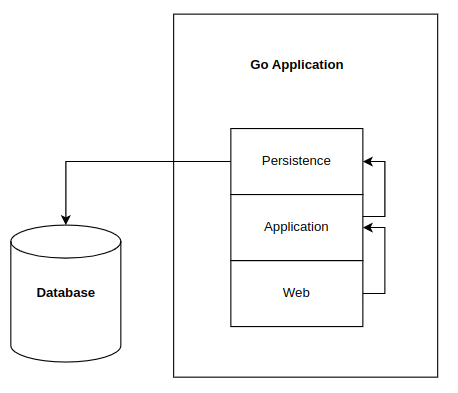
\includegraphics[width=0.8\linewidth]{report/images/system_architecture.png}
    \caption{MiniTwit Architecture}
    \label{fig:minitwit}
\end{figure}

The application is implemented using the RESTful API, which means that when a user interacts with a part of the 
view, an HTTP request containing a new state of the application is sent. This request is then handled by the corresponding controller, and it ensures 
that the correct action is taken. This could be a call to a function that updates the model, and the return of 
an appropriate HTTP response. 


\subsection{Dependencies of MiniTwit system}

For the MiniTwit application to run we are depending on first and foremost Digital Oecan whos servers the application is 
hosted on. The servers are running 9 docker containers responsible for: 
\begin{itemize}
    \item The Database running on a postgres:14.1-alpine image - Responsible for holding all the users data.
    \item The Server itself running on a golang:bullseye image.
    \item A reddis server for storing sessions and the integer 'latest'.
    \item Elastic Search - Indexing logs such that we can search and analyse them
    \item Filebeat for collecting and forwarding the logging to Elastic search
    \item Kibana for visualizing the results from Elastic search
    \item Prometheus for monitoring the application in terms of CPU usage and request time
    \item Grafana for visualizing the monitoring
    \item Nginx for load balancer? skriv her
\end{itemize}

From within each of these containers we depend on large number of libraries of which the major ones we consider to be:
\begin{itemize}
    \item Gorm used for object-relational mapping allowing us to perfom CRUD opertations io GO.
    \item Gin handeling all of the routing of the HTTP methods.
    \item x/crypto/bcrypt libaray for hashing the user password.
\end{itemize}

In a more board term of sense we also depend on Docker, Go and SSH protocol to work. We choose Go for the reason being 
that \todo{skriv her} 

At last we also depend on pre-build git workflows such as \textit{docker/build-push-action@v2} or \textit{rymndhng/release-on-push-action@master}.

%OBS MSc students: Remember to log and provide good arguments for the choice of ORM framework and chosen DBMS.

%OBS MSc students: Remember to log and provide good arguments for the choice of programming language and framework

%OBS MSc students: Remember to log and provide good arguments for the choice of virtualization techniques and deployment targets

% Argue for Terraform choice??

% deployment diagram??

%%% NOTE:
%The application is hosted at Digital Ocean. We use Docker Swarms to scale the application horizontally. For 
%monitoring the application we use Grafana. Logging is done using Elastic Search and Kibana. Additionally, we have a Redis database 
%that stores sessions and the integer 'latest' and a postgreSQL database storing other information, such as 
%the registered users and created messages. 

\subsection{Important Interactions of Subsystems}

\subsection{Current state of the system}

\subsection{Project License}